%%
%% This is file `tikzposter-template.tex',
%% generated with the docstrip utility.
%%
%% The original source files were:
%%
%% tikzposter.dtx  (with options: `tikzposter-template.tex')
%%
%% This is a generated file.
%%
%% Copyright (C) 2014 by Pascal Richter, Elena Botoeva, Richard Barnard, and Dirk Surmann
%%
%% This file may be distributed and/or modified under the
%% conditions of the LaTeX Project Public License, either
%% version 2.0 of this license or (at your option) any later
%% version. The latest version of this license is in:
%%
%% http://www.latex-project.org/lppl.txt
%%
%% and version 2.0 or later is part of all distributions of
%% LaTeX version 2013/12/01 or later.
%%


\documentclass{tikzposter} %Options for format can be included here

\usepackage{todonotes}

\usepackage[tikz]{bclogo}
\usepackage{lipsum}
\usepackage{amsmath}

\usepackage{booktabs}
\usepackage{longtable}
\usepackage[absolute]{textpos}
\usepackage[it]{subfigure}
\usepackage{graphicx}
\usepackage{cmbright}
%\usepackage[default]{cantarell}
%\usepackage{avant}
%\usepackage[math]{iwona}
\usepackage[math]{kurier}
\usepackage[T1]{fontenc}


%% add your packages here
\usepackage{hyperref}
% for random text
\usepackage{lipsum}
\usepackage[english]{babel}
\usepackage[pangram]{blindtext}

%wmx add under:

\usepackage{caption}
\usepackage{float}


\colorlet{backgroundcolor}{blue!10}

% Title, Author, Institute
\title{FILP 00 FINAL REPORT}
\author{Mingxi Wang}
\institute{ Jilin University, China \\
}
%\titlegraphic{logos/tulip-logo.eps}

%Choose Layout
\usetheme{Wave}

%\definebackgroundstyle{samplebackgroundstyle}{
%\draw[inner sep=0pt, line width=0pt, color=red, fill=backgroundcolor!30!black]
%(bottomleft) rectangle (topright);
%}
%
%\colorlet{backgroundcolor}{blue!10}

\begin{document}
	
	
	\colorlet{blocktitlebgcolor}{blue!23}
	
	% Title block with title, author, logo, etc.
	\maketitle
	
	\begin{columns}
		% FIRST column
		\column{0.5}% Width set relative to text width
		
		%%%%%%%%%% -------------------------------------------------------------------- %%%%%%%%%%
		%\block{Main Objectives}{
		%  	      	\begin{enumerate}
		%  	      	\item Formalise research problem by extending \emph{outlying aspects mining}
		%  	      	\item Proposed \emph{GOAM} algorithm is to solve research problem
		%  	      	\item Utilise pruning strategies to reduce time complexity
		%  	      	\end{enumerate}
		%%  	      \end{minipage}
		%}
		%%%%%%%%%% -------------------------------------------------------------------- %%%%%%%%%%
		
		
		%%%%%%%%%% -------------------------------------------------------------------- %%%%%%%%%%
		\block{Introduction}{
			\begin{description}
				\item[Project objectives] :\\
				The project analyzed 12 years of crime reports from all of San Francisco's neighborhoods to create a model that can predict crime categories at a \emph{given time and place}.
				
				\item[Project background] :\\
				Crime is a kind of behavior that does great harm to the society. It brings great loss of life and property to human beings.In modern society, human beings prevent crime through strict judicial means, and research on crime prevention based on sociology, psychology and law.The objective of this project is to quantitatively analyze a data set of nearly 12 years of crime reports from all San Francisco neighborhoods by computer means and to create a model that predicts the type of crime that will occur given information such as \emph{time and location}.
			\end{description}
			
		}
		%%%%%%%%%% -------------------------------------------------------------------- %%%%%%%%%%
		
		
		%%%%%%%%%% -------------------------------------------------------------------- %%%%%%%%%%
		\block{Research contents and methods}{
			\begin{itemize}
				\item
				%\emph{Group Outlying Aspects Mining}
				\textbf{Evaluation metric}
				Multi-class logarithmic loss, which measures that the model output is a probability value between 0 and 1.
				
				\item
				\textbf{Data cleaning}
				There are 2323 duplicate items that need to be removed
				Throw away samples in a range of longitude and latitude (e.g., 50)
				
				\item
				\textbf{Characteristics of the engineering}
				The features are analyzed and processed to obtain more suitable features for model input.
				
				\item
				\textbf{Information coding}
				The discrete data is converted to a number between 0 and N-1, where N is the number of different values in a list.You can think of it as the number of different values of a feature.
				
				\item
				\textbf{Training model}
				Train 23 Epochs.
				Use cross validation to evaluate the quality of our model.    
				
			\end{itemize}
			
		}
		%%%%%%%%%% -------------------------------------------------------------------- %%%%%%%%%%
		
		
		%%%%%%%%%% -------------------------------------------------------------------- %%%%%%%%%%
		
		%\note{Note with default behavior}
		
		%\note[targetoffsetx=12cm, targetoffsety=-1cm, angle=20, rotate=25]
		%{Note \\ offset and rotated}
		
		% First column - second block
		
		
		%%%%%%%%%% -------------------------------------------------------------------- %%%%%%%%%%
		
		
		\block{Data Visualization}{
			
			%	\begin{center}
			%		\begin{figure}[htbp]
			%			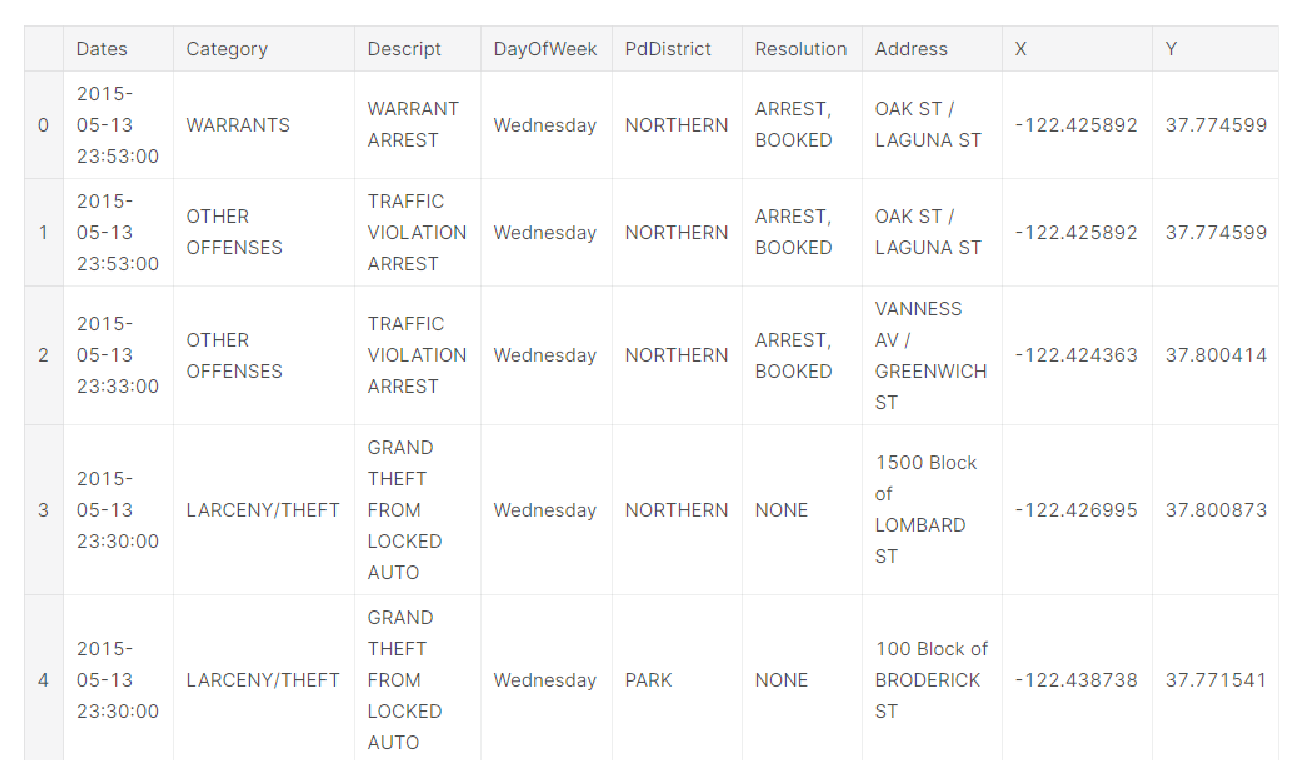
\includegraphics[scale=0.6]{pic/qmyangben.eps}
			%			\caption{preview}
			%		\end{figure}
			%	\end{center}
			\begin{center}
				\includegraphics[scale=1.1]{pic/qmshuxingtu.eps}\\
			\end{center}
			\begin{center}
				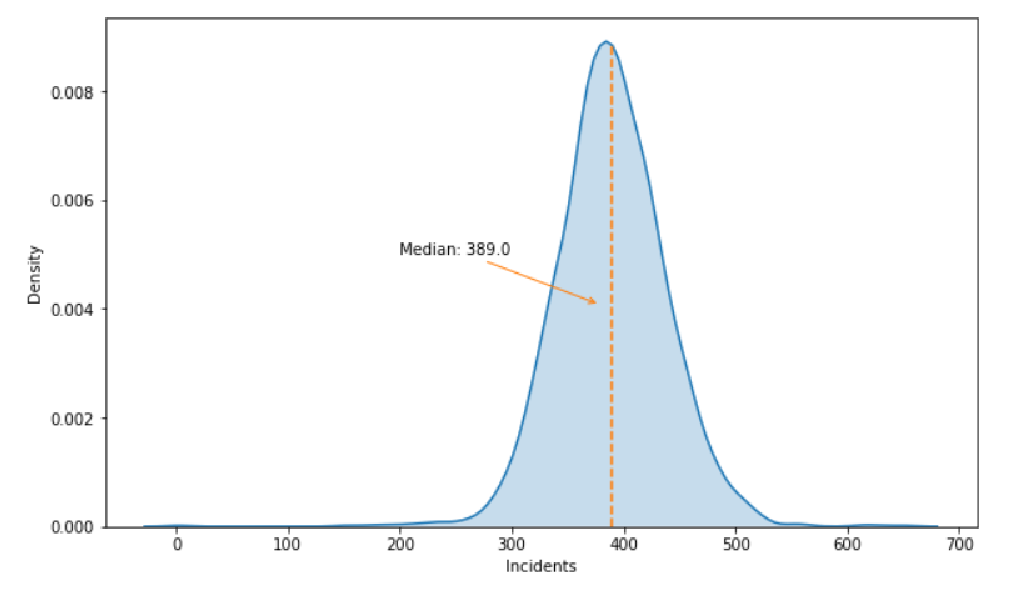
\includegraphics[scale=1.1]{pic/qmzhengtai.eps}\\
			\end{center}
			\begin{center}
				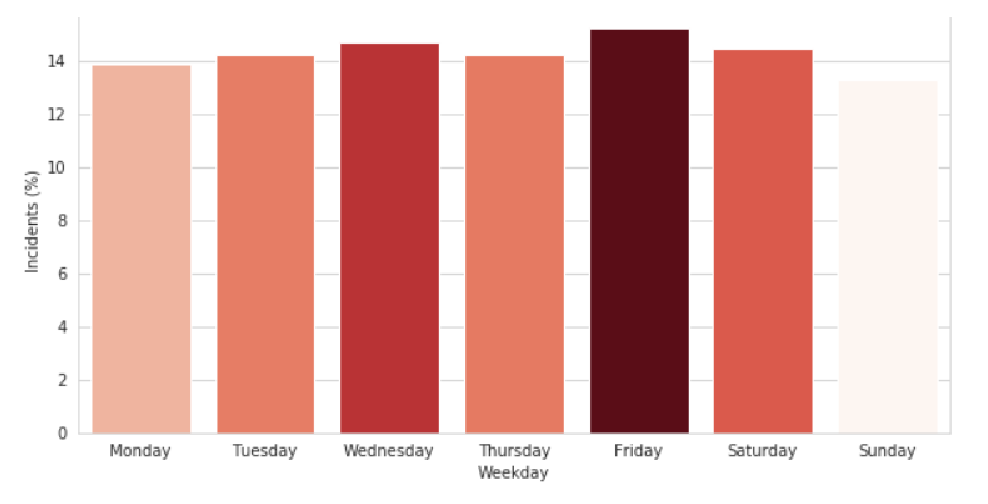
\includegraphics[scale=1.1]{pic/qmzhifangtu.eps}\\
			\end{center}
			%\includegraphics[scale=0.6]{pic/qmzhexiantu.eps}\\
		}
		%%%%%%%%%% -------------------------------------------------------------------- %%%%%%%%%%
		
		
		% SECOND column
		\column{0.5}
		%Second column with first block's top edge aligned with with previous column's top.
		
		%%%%%%%%%% -------------------------------------------------------------------- %%%%%%%%%%
		\block{The data analysis}{
			The graph shows the average number of incidents per hour for the five crime categories.Obviously, different crimes occur with different frequencies at different times of the day.Prostitution, for example, takes place mostly at night, gambling incidents take place from late at night until morning, and burglaries from early morning until afternoon.As before, this is clear evidence that time parameters will also play an important role.
			\begin{center}
				\includegraphics[scale=1.6]{pic/qmzhexiantu.eps}\\
			\end{center}
		}
		%%%%%%%%%% -------------------------------------------------------------------- %%%%%%%%%%
		% Second column - first block
		
		
		%%%%%%%%%% -------------------------------------------------------------------- %%%%%%%%%%
		\block[titleleft]{Architecture of the model}
		{
			We describe the architecture of the model in a circular and iterative manner, as described in the following six points:\\
			\\
			1. Make the decision tree fit the data\\
			2. Evaluation model\\
			3. Add weight to incorrect samples\\
			4. Select the leaf nodes with the greatest incremental loss for growth\\
			5. Generate the tree at the node in the previous step\\
			6. Go to Step 2 for the cycle\\
		}
		%%%%%%%%%% -------------------------------------------------------------------- %%%%%%%%%%
		
		
		% Second column - second block
		%%%%%%%%%% -------------------------------------------------------------------- %%%%%%%%%%
		\block[titlewidthscale=1, bodywidthscale=1]
		{Conclusion}
		{
			Our training model has gone through 23 EPOCH cycles, and achieved good results on both the training set and the test set.The resulting loss value score is about 2.4, which is a good score compared to other models.\\
			\\
			Although the model performs well, there is still room for improvement.The model performance will be further improved in the future
		}
		%%%%%%%%%% -------------------------------------------------------------------- %%%%%%%%%%
		
		
		% Bottomblock
		%%%%%%%%%% -------------------------------------------------------------------- %%%%%%%%%%
		\colorlet{notebgcolor}{blue!20}
		\colorlet{notefrcolor}{blue!20}
		\note[targetoffsetx=8cm, targetoffsety=-14cm, angle=30, rotate=15,
		radius=2cm, width=.26\textwidth]{
			Acknowledgement
			\begin{itemize}
				\item
				International Cooperation Project (Y7Z0511101)
				of IIE,
				Chinese Academy of Sciences
			\end{itemize}
		}
		
		%\note[targetoffsetx=8cm, targetoffsety=-10cm,rotate=0,angle=180,radius=8cm,width=.46\textwidth,innersep=.1cm]{
		%Acknowledgement
		%}
		
		%\block[titlewidthscale=0.9, bodywidthscale=0.9]
		%{Acknowledgement}{
		%}
		%%%%%%%%%% -------------------------------------------------------------------- %%%%%%%%%%
		
	\end{columns}
	
	
	%%%%%%%%%% -------------------------------------------------------------------- %%%%%%%%%%
	%[titleleft, titleoffsetx=2em, titleoffsety=1em, bodyoffsetx=2em,%
	%roundedcorners=10, linewidth=0mm, titlewidthscale=0.7,%
	%bodywidthscale=0.9, titlecenter]
	
	%\colorlet{noteframecolor}{blue!20}
	\colorlet{notebgcolor}{blue!20}
	\colorlet{notefrcolor}{blue!20}
	\note[targetoffsetx=-13cm, targetoffsety=-44cm,rotate=0,angle=180,radius=8cm,width=.96\textwidth,innersep=.4cm]
	{
		\begin{minipage}{0.3\linewidth}
			\centering
			
\includegraphics[width=24cm]{logos/tulip-wordmark.eps}
		\end{minipage}
		\begin{minipage}{0.7\linewidth}
			{ \centering
				The $11^{th}$ International Conference on Knowledge Science,
				Engineering and Management (KSEM 2018),
				17-19/08/2018, Changchun, China
			}
		\end{minipage}
	}
	%%%%%%%%%% -------------------------------------------------------------------- %%%%%%%%%%
	
	
\end{document}

%\endinput
%%
%% End of file `tikzposter-template.tex'.
